\documentclass[letterpaper,final,12pt,reqno]{amsart}

\usepackage[total={6.3in,9.2in},top=1.1in,left=1.1in]{geometry}

\usepackage{times,bm,bbm,empheq,fancyvrb,graphicx,amsthm,amssymb}
\usepackage[dvipsnames]{xcolor}
\usepackage{longtable}
\usepackage{booktabs}

\usepackage{tabto}
\TabPositions{1.5cm}

\usepackage{tikz}
\usetikzlibrary{decorations.pathreplacing}

\usepackage[kw]{pseudo}
\pseudoset{%
left-margin=15mm,%
topsep=5mm,%
label=\footnotesize\arabic*,%
idfont=\texttt,%
ctfont=\textsl,%
ct-left=\qquad\qquad(,%
ct-right=),%
}

\usepackage{float}

% hyperref should be the last package we load
\usepackage[pdftex,
colorlinks=true,
plainpages=false, % only if colorlinks=true
linkcolor=blue,   % ...
citecolor=Red,    % ...
urlcolor=black    % ...
]{hyperref}

\renewcommand{\baselinestretch}{1.05}

\allowdisplaybreaks[1]  % allow display breaks in align environments, if they avoid major underfulls

\newtheoremstyle{cstyle}% name
  {5pt}% space above
  {5pt}% space below
  {\itshape}% body font
  {}% indent amount
  {\itshape}% theorem head font
  {.}% punctuation after theorem head
  {.5em}% space after theorem head
  {\thmname{#1}\thmnumber{ #2}\thmnote{ (#3)}}% theorem head spec
\theoremstyle{cstyle}

\newtheorem{theorem}{Theorem}
\newtheorem{lemma}[theorem]{Lemma}
\newtheorem{assumptions}[theorem]{Assumptions}

\newtheoremstyle{cstyle*}% name
  {5pt}% space above
  {5pt}% space below
  {\itshape}% body font
  {}% indent amount
  {\itshape}% theorem head font
  {.}% punctuation after theorem head
  {.5em}% space after theorem head
  {\thmname{#1}}% theorem head spec
\theoremstyle{cstyle*}
\newtheorem{assumptions*}{Assumptions}

\newtheoremstyle{dstyle}% name
  {5pt}% space above
  {5pt}% space below
  {}%{\itshape}% body font
  {}% indent amount
  {\itshape}% theorem head font
  {.}% punctuation after theorem head
  {.5em}% space after theorem head
  {\thmname{#1}\thmnumber{ #2}\thmnote{ (#3)}}% theorem head spec
\theoremstyle{dstyle}

\newtheorem{definition}[theorem]{Definition}
\newtheorem{example}[theorem]{Example}

%% numbering
%\numberwithin{equation}{section}
%\numberwithin{figure}{section}
%\numberwithin{table}{section}
%\numberwithin{theorem}{section}

\newcommand{\eps}{\epsilon}
\newcommand{\RR}{\mathbb{R}}

\newcommand{\grad}{\nabla}
\newcommand{\Div}{\nabla\cdot}
\newcommand{\trace}{\operatorname{tr}}

\newcommand{\hbn}{\hat{\mathbf{n}}}

\newcommand{\bb}{\mathbf{b}}
\newcommand{\be}{\mathbf{e}}
\newcommand{\bbf}{\mathbf{f}}
\newcommand{\bg}{\mathbf{g}}
\newcommand{\bn}{\mathbf{n}}
\newcommand{\br}{\mathbf{r}}
\newcommand{\bu}{\mathbf{u}}
\newcommand{\bv}{\mathbf{v}}
\newcommand{\bw}{\mathbf{w}}
\newcommand{\bx}{\mathbf{x}}
\newcommand{\by}{\mathbf{y}}
\newcommand{\bz}{\mathbf{z}}

\newcommand{\bF}{\mathbf{F}}
\newcommand{\bV}{\mathbf{V}}
\newcommand{\bX}{\mathbf{X}}

\newcommand{\bxi}{\bm{\xi}}
\newcommand{\bzero}{\bm{0}}

\newcommand{\cK}{\mathcal{K}}
\newcommand{\cV}{\mathcal{V}}

\newcommand{\rhoi}{\rho_{\text{i}}}

\newcommand{\ip}[2]{\left<#1,#2\right>}

\newcommand{\maxR}{R^{\bm{\oplus}}}
\newcommand{\minR}{R^{\bm{\ominus}}}
\newcommand{\iR}{R^{\bullet}}

\newcommand{\nn}{{\text{n}}}
\newcommand{\pp}{{\text{p}}}
\newcommand{\qq}{{\text{q}}}
\newcommand{\rr}{{\text{r}}}

\newcommand{\supp}{\operatorname{supp}}
\newcommand{\Span}{\operatorname{span}}


\begin{document}
\title[A linear model for the coupled equations of glacier evolution]{A linear model for the coupled equations \\ of glacier evolution}

\author{Ed Bueler}

\date{\today}

\begin{abstract} FIXME
\end{abstract}

\maketitle

%\tableofcontents

\thispagestyle{empty}
%\bigskip

\newfloat{pseudofloat}{t}{xyz}[section]
\floatname{pseudofloat}{Algorithm}


\section{Introduction} \label{sec:intro}

FIXME

\section{Model equations} \label{sec:model}

Our model problem is a 2D equation with both partial derivatives and integrals, namely equation \eqref{eq:modelproblem} below, but it is created from looking at a notional surface process on the top of a 3D domain.  We start with this 3D problem.

For length $L>0$ and height $H>0$ given, let $\Omega = (0,L)^2\times (0,H)$ be the rectangular-solid in 3D.  On $\Omega$ the coordinates are $x,y,z$ with $0<x,y<L$ and $0<z<H$.  We call the $z=0$ boundary the \emph{bottom} and the $z=H$ boundary the \emph{top}.  The remaining boundary parts are the \emph{sides}.  Let $g(x,y)$ be a given function on the top, i.e.~defined for $0<x,y<L$.  We consider the following 3D Laplace equation problem for the scalar solution $u(x,y,z)$ defined on $\Omega$:
\begin{subequations}
\label{eq:laplaceproblem}
\begin{align}
\grad^2 u &= 0 & &\text{in } \Omega = (0,L)^2\times (0,H), \\
u &= 0 & &\text{on the bottom and sides}, \\
\frac{\partial u}{\partial z} &= g & &\text{on the top $z=H$}.
\end{align}
\end{subequations}
Note that $\frac{\partial u}{\partial n}=\frac{\partial u}{\partial z}$ is the outward-normal derivative on the top.  See Figure \ref{fig:laplaceproblem}.

\begin{figure}[ht]
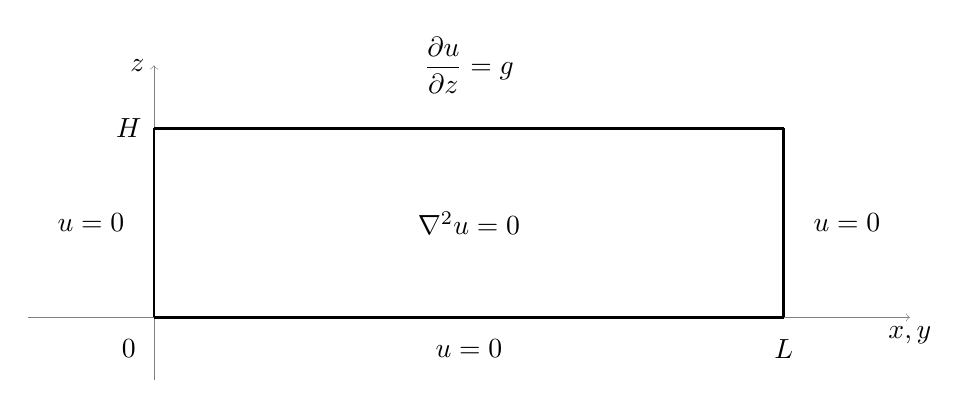
\begin{tikzpicture}[scale=8.0]
  % axes; x,y are horizontal and z is vertical
  \draw[->,gray,very thin] (-0.2,0.0) -- (1.2,0.0) node[below,black] {$x,y$};
  \draw[->,gray,very thin] (0.0,-0.1) -- (0.0,0.4) node[left,black] {$z$};
  % R = (0,L)^2
  \node at (-0.04,-0.05) {$0$};
  \node at (1.0,-0.05) {$L$};
  \node at (-0.04,0.3) {$H$};
  \draw[line width=1.0pt] (0.0,0.0) -- (0.0,0.3);
  \draw[line width=1.0pt] (1.0,0.0) -- (1.0,0.3);
  \draw[line width=1.0pt] (0.0,0.0) -- (1.0,0.0);
  \draw[line width=1.0pt] (0.0,0.3) -- (1.0,0.3);
  % equation and boundary conditions
  \node at (0.5,0.15) {$\grad^2 u = 0$};
  \node at (0.5,-0.05) {$u=0$};
  \node at (0.5,0.4) {$\displaystyle \frac{\partial u}{\partial z} = g$};
  \node at (-0.1,0.15) {$u=0$};
  \node at (1.1,0.15) {$u=0$};
\end{tikzpicture}
\caption{Laplace equation problem \eqref{eq:laplaceproblem} uniquely defines $u(x,y,z)$ if $g(x,y)$ is a given top-surface Neumann condition.}
\label{fig:laplaceproblem}
\end{figure}

It is well-known that Laplace equation problem \eqref{eq:laplaceproblem} has a unique solution $u$ if $g$ is minimally well-behaved \cite{Elmanetal2014,Evans2010}.  The problem has a mixture of homogeneous Dirichlet (bottom and sides) and nonhomogeneous Neumann (top) boundary conditions, and the fact that  Dirichlet conditions apply on a positive-measure part of the boundary\footnote{In \eqref{eq:laplaceproblem}, Dirichlet conditions apply on quite a large part of the boundary, in fact, namely 5 of 6 faces!} implies uniqueness.

Thus it is reasonable to talk about \emph{the} solution $u$ of \eqref{eq:laplaceproblem} for given top-surface Neumann data $g$, and in particular to consider the well-defined map from $g(x,y)$ to the top-surface values of the solution $u(x,y,H)$.  This is a linear \emph{Neumann-to-Dirichlet map},
\begin{equation}
N : \, g(x,y) \, \mapsto \, u(x,y,H).  \label{eq:ntod}
\end{equation}
As shown in the Appendix, a separation of variables argument allows us to express this map as an integral against a know \emph{kernel} $K$, namely
\begin{equation}
(N g)(x,y) = u(x,y,H) = \int_0^L \int_0^L K(x,y;\xi,\eta)\, g(\xi,\eta)\,d\xi\,d\eta  \label{eq:ntodformula}
\end{equation}
where
\begin{equation}
K(x,y;\xi,\eta) = (\text{FIXME: a sum of $\sin() \sinh()$ products; closed form?})  \label{eq:kernelformula}
\end{equation}

FIXME model problem is on 2D domain $R = (0,L)^2$, with $\eps>0$:
\begin{equation}
-\eps \grad^2 s + \frac{N s}{H} = f  \label{eq:modelproblem}
\end{equation}
See Figure \ref{fig:modelproblem}.

\begin{figure}
\begin{tikzpicture}[scale=5.0]
  % axes
  \draw[->,gray,very thin] (-0.2,0.0) -- (1.2,0.0) node[below,black] {$x$};
  \draw[->,gray,very thin] (0.0,-0.2) -- (0.0,1.2) node[left,black] {$y$};
  % R = (0,L)^2
  \node at (-0.04,-0.05) {$0$};
  \node at (1.0,-0.05) {$L$};
  \node at (-0.04,1.0) {$L$};
  \draw[line width=1.0pt] (0.0,0.0) -- (0.0,1.0);
  \draw[line width=1.0pt] (1.0,0.0) -- (1.0,1.0);
  \draw[line width=1.0pt] (0.0,0.0) -- (1.0,0.0);
  \draw[line width=1.0pt] (0.0,1.0) -- (1.0,1.0);
  % equation and boundary conditions
  \node at (0.5,0.5) {$\displaystyle -\eps \grad^2 s + \frac{N s}{H} = f$};
  \node at (0.5,-0.1) {$s=0$};
  \node at (0.5,1.1) {$s=0$};
  \node[rotate=90] at (-0.1,0.5) {$s=0$};
  \node[rotate=-90] at (1.1,0.5) {$s=0$};
\end{tikzpicture}
\caption{Model problem \eqref{eq:modelproblem} on $R = (0,L)^2$.}
\label{fig:modelproblem}
\end{figure}

FIXME alternative model has ``$N(\grad s)$'' instead, in some form

FIXME observe how $H^{-1} Ns$ behaves as $H\to 0$

FIXME much more to write

\section{On multigrid solutions of \eqref{eq:modelproblem}} \label{sec:numerical}

FIXME \cite{Briggsetal2000,Bueler2021,Trottenbergetal2001} for multigrid

FIXME need to explore smoothers which can handle the $N$ operator

\section{Discussion and Conclusion} \label{sec:conclusion}

FIXME \cite{Girouardetal2022} show that the Neumann-to-Dirichlet map $\mathcal{N}:\frac{\partial u}{\partial n}|_{\partial} \mapsto u|_{\partial}$ along the \emph{entire} boundary of a 3D domain $\Omega \subset \RR^3$ is very close to $|\grad_{\partial}|^{-1}$ where $|\grad_{\partial}| = \sqrt{-\grad_{\partial}^2}$ is the square root of the positive boundary Laplacian $-\grad_{\partial}^2$; they are identical only when $\Omega$ is a 3D sphere, which is not true here

\bibliography{model}
\bibliographystyle{siam}


%\appendix
%\section{FIXME}

\end{document}

